\section{Methodology}
In this section, we outline the methodology employed to gather, process, and annotate the data for our study. We begin by detailing the sources of our multimodal video data and personality labels, focusing on how we efficiently align subtitles with original scripts to ensure accurate temporal and character associations. And we also present our annotation process, explaining how we leverage the ChatGPT API to automatically annotate social and emotional relations among characters within the text data. 
\subsection{Source of Data}
Our data source contains mainly two parts, the multimodal video data and personality labels. For video data, we include 14 different genres of TV series and movies via an open-source website\footnote[1]{\href{https://yts.mx/}{https://yts.mx/}}, and for the scripts and subtitles, we also find other open-source websites\footnote[2]{\href{https://www.simplyscripts.com/}{https://www.simplyscripts.com/}}\footnote[3]{\href{https://subscene.com/}{https://subscene.com/}} for research offering the free scripts and subtitles of many famous movie and television programs. Considering the insufficient labeling method of existing works, we collect the personality annotations from personality database website as well as the voting distribution and align them to correctly scripts. 
\subsection{Data Alignment Process}
As subtitle contain temporal information and original scripts associate utterances with characters, we are supposed to align them properly as efficient as possible. However, most of the existing multimodal datasets annotate the timestamps manually with taking up a great deal of time. There are also some works which utilize different automatic tools to align the utterances with their corresponding information. For instance, \citet{lian2024merbench} use an Automatic Sound Recognition (ASR) tool called Gentle\footnote[4]{\href{https://github.com/lowerquality/gentle}{https://github.com/lowerquality/gentle}} to get the timestamps for the utterances. To streamline the process of aligning dialogue utterances with their respective timestamps and speakers from subtitles, we propose an efficient method leveraging a fuzzy matching algorithm (see Appendix \ref{sec:appendixC}). 
Following successful alignment, we proceed to segment the video content into distinct scenes according to the timestamps. Besides, we use FFmpeg\footnote[1]{\href{https://ffmpeg.org/}{https://ffmpeg.org/}} to extract the audio track from the video clips and output it as a \textit{.mp3} file.


\begin{figure}[ht]
    \small
    \centering 	 	 	 	
    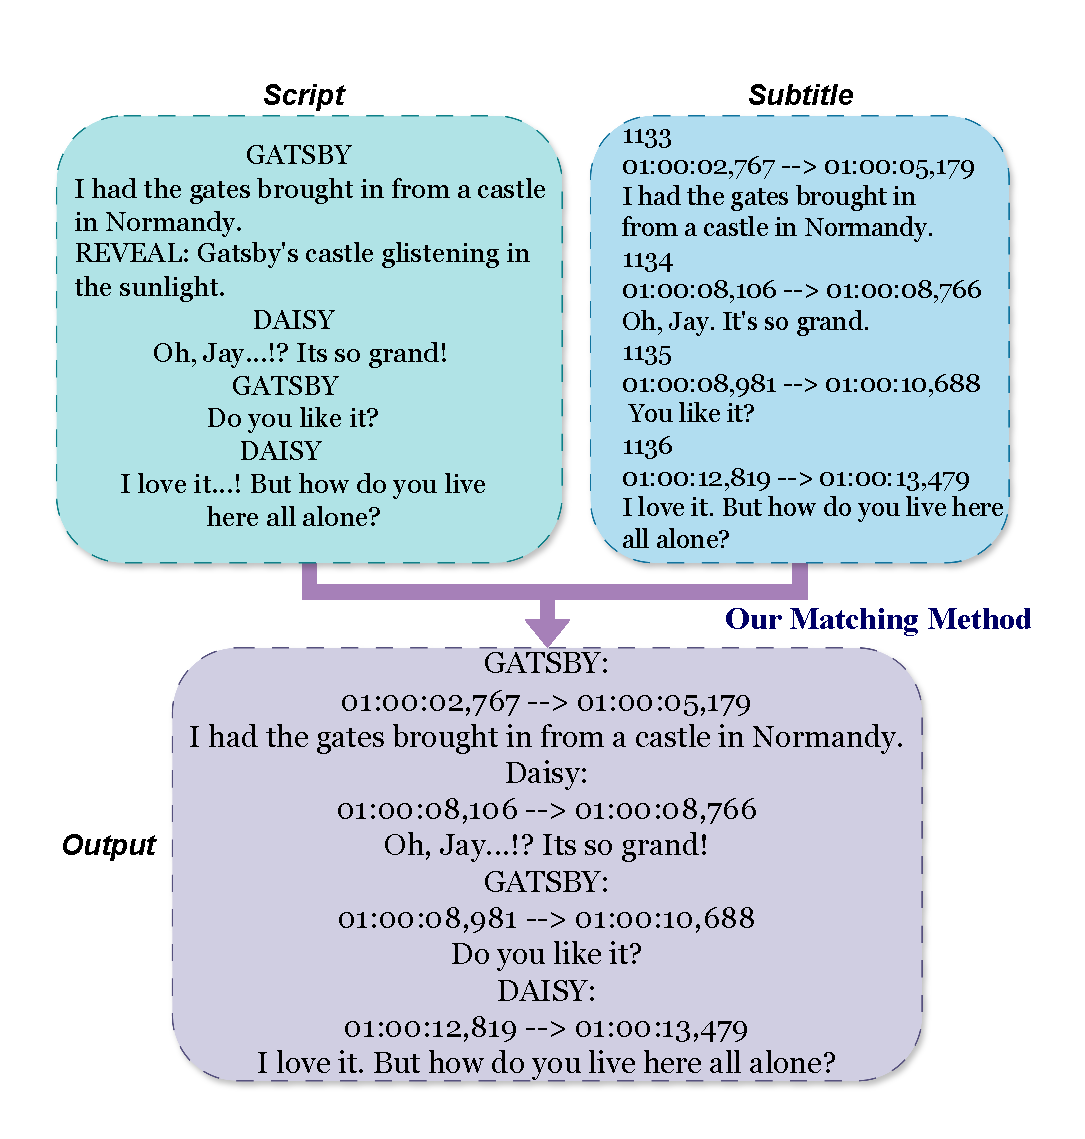
\includegraphics[width=\linewidth, trim= 0 10 0 10, clip]{images/raw_data.pdf}
	\caption{Process of data alignment}
    \label{fig:alig}
\end{figure}

\subsection{Annotation Process}

We construct a process to automatically annotate the social and emotion relations among characters by using ChatGPT API~\citep{openai2023gpt35}. Only text data are supposed to be processed, thus we choose \textit{gpt-3.5-turbo-1106} pre-trained model to annotate our dataset. Since we preprocess the text data and divide them into scenes, we design a prompt to ask ChatGPT for identifying both social and emotion relations for every single scene. When annotating our data, we encounter a challenge in representing unidirectional affectionate relationships, where A likes B, but B does not reciprocate the feelings. While social relations do not present this issue, emotion relations require a solution to capture this directional information. We address this by interpreting the relative position of different characters in the tuple. For example, A and B (family, fondness) indicates that A has positive feelings towards B. Conversely, if B has positive feelings towards A, the tuple would be B and A, (family, fondness). This approach allows us to clearly represent the directionality of emotional relations.

Based on the definitions of relations, we design this prompt for relations annotation (Fig \ref{fig:prompt}). The prompt categorizes relations into seven social and eight emotion types, ensuring comprehensive coverage of human interactions. Note that we require ChatGPT to generate the responses following our format strictly so that we could better manipulate them flexibly. 

\begin{figure}[ht]
	\centering
	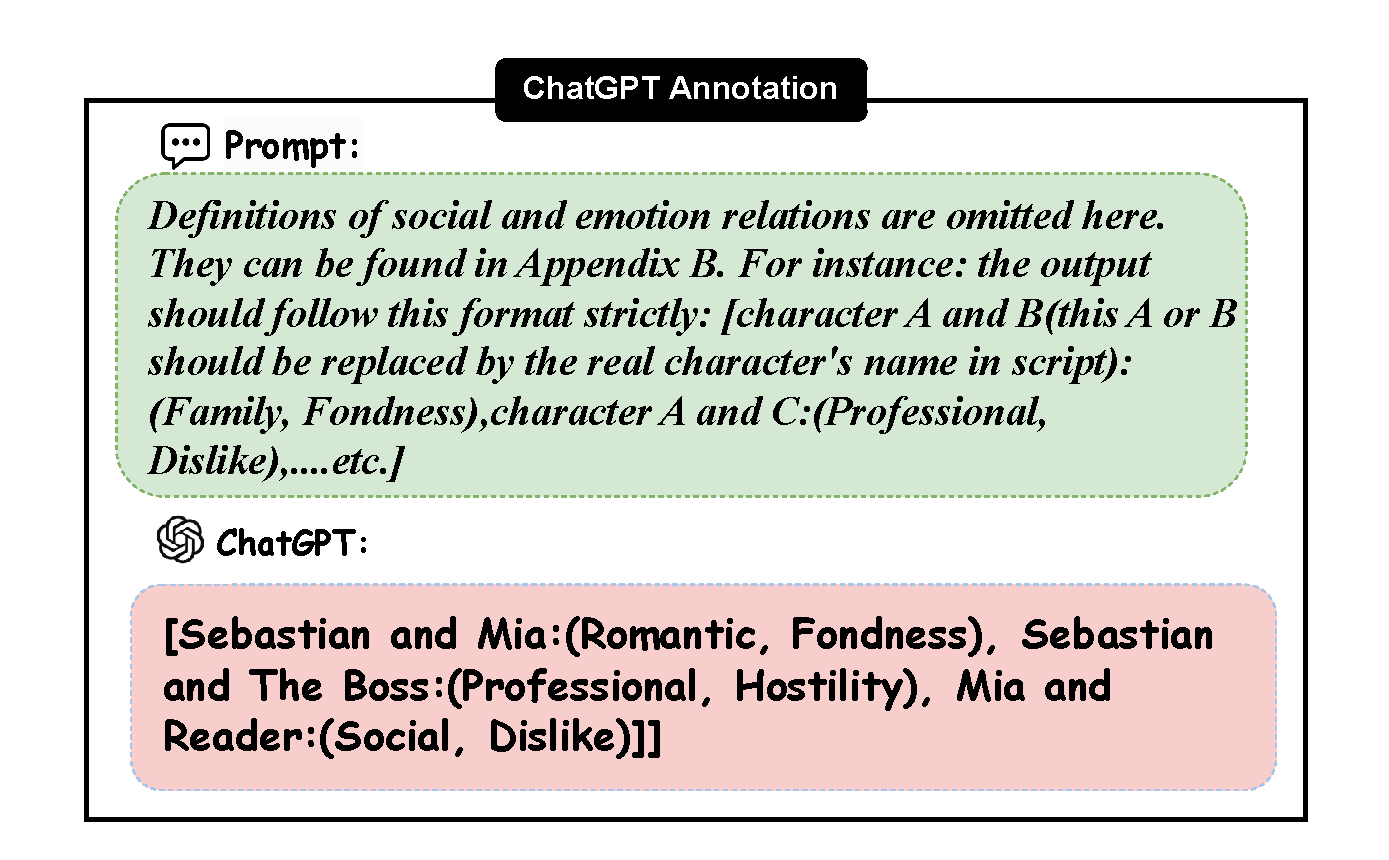
\includegraphics[width=\linewidth]{images/prompt.pdf}
	\caption{Prompt design for relations annotation}
	\label{fig:prompt}
\end{figure}

